%!TEX root=../../root.tex

\section{Lezione 18}

\subsection{Complessità di una TM che simula una NTM}

Precedentemente si è indagata l'equivalenza tra macchine di Turing $TM$ e macchine di Turing non deterministiche $NTM$. In particolare sappiamo che 
\[
	T \in NTM \implies \exists \ T' \in TM \text{ tale che } L(T) = L(T')
\]

Cosa possiamo dire dal punto di vista della complessità? Ovvero data $T \in NTM$ e $t_T(n)$ e una $T' \in TM$ equivalente, cosa possiamo dire di $t_{T'}(n)$?

Senza perdere di generalità, assumiamo che $T$ abbia un massimo grado di non determinismo pari a 2, in quanto il ragionamento vale per qualsiasi $k$. Con questa assunzione, l'albero delle configurazioni della $NTM$ è binario. Per definizione di $t_T(n)$, essa è il massimo numero di mosse che la macchina $T$ compie su input di dimensione $n$; di conseguenza per una $NTM$ essa coincide con l'altezza dell'albero, in quanto ogni cammino radice foglia è costituito da al massimo $t_T(n)$ mosse che una "copia" della macchina compie sull'input.

L'albero ha quindi al massimo $2^{t_T(n)}$  foglie, ovvero la $TM$ che simula ha $2^{t_T(n)}$ cammini radice foglia da simulare. Ognuna di queste simulazioni richiede al più $t_T(n)$ mosse. Da queste considerazioni discende che
\[
	t_{T'}(n) = t_{T}(n) \cdot 2^{t_T(n)} = 2^{log(t_T(n))} \cdot 2^{t_T(n)} = 2^{t_T(n) + log(t_T(n))} = 2^{O(t_T(n))}
\]
ovvero una macchina di Turing impiega tempo esponenziale per simulare il non determinismo.

\subsection{La classe NP}

Definiamo $NTIME(n^k)$ l'insieme dei linguaggi per cui esiste una $NTM$ che ne accetta le parole di dimensione $n$ in un numero di passi $O(n^k)$:

\[
	NTIME(n^k) = \{ L \ | \ \exists \ T \in NTM \text{ tale che } L(T) = L \text{ e } t_T(n) = O(n^k) \}
\]

Sulla base di questa definizione introduciamo la classe dei linguaggi (o equivalentemente dei \textit{problemi}) $NP$:
\[
	NP = \bigcup_{k \geq 0} \{ NTIME(n^k) \}
\]

Essa \textit{non} è composta dai problemi non risolvibili polinomialmente, in quanto quella descrizione individua la classe $\overline{P}$. 
\\
Invece di $NP$ fanno parte problemi che si è in grado di risolvere in tempo polinomiale tramite \textit{non determinismo}. Della maggior parte di essi non si ha la certezza che non sia possibile costruire una macchina di Turing, ovvero un algoritmo, che deterministicamente li risolva in tempo polinomiale. Semplicemente un tale algoritmo non è ancora stato trovato.

\subsection{Problemi NP}

\subsubsection{Problema del Cammino hamiltoniano}

\[
	HAMPATH = \{ <G, s, t> \ | \ G \text{ è un grafo diretto con un c.h. da } s \text{ a } t\}
\]

Indichiamo con \textit{c.h.} per brevità un \textit{cammino hamiltoniano}, ovvero una sequenza di nodi $v_1,...,v_n$, dove $n = |V_G|$, con le seguenti proprietà:
\begin{itemize}
	\item $v_1 = s$ e $v_n = t$
	\item $(v_i, v_{i+1}) \in E_G$ per $i = 1, ..., n-1$
\end{itemize}

Per mostrare che $HAMPATH \in NP$, esibiamo una $NTM$ che lo decide in tempo polinomiale.
\\

$T_{HP}$
\begin{description}
	\item \textit{input}: $<G, s, t>$

	\item \textit{output}: SÌ se $<G,s,t> \in HAMPATH$, NO altrimenti

	\item \textit{descrizione}:
	\begin{enumerate}[label*=\arabic*.]
		\item Genera \textit{non deterministicamente} una permutazione $v_1, ..., v_n$ dei nodi di $G$

		\item Verifica che la permutazione generata sia effettivamente un c.h. nel seguente modo:
		\begin{enumerate}[label*=\arabic*.]
			\item Verifica che $v_1$ sia uguale a $s$ e che $v_n$ sia uguale a $t$
			\item Per ogni $v_i, v_{i+1}$ nella permutazione, verifica che vi sia l'arco $(v_i, v_{i+1}) \in E_G$
		\end{enumerate}
	\end{enumerate}
\end{description}

\paragraph{Complessità} Prima di tutto, vediamo come costruire una $NTM$ che genera permutazioni su $\{1, ..., n\}$. Modificando leggermente la macchina che descriveremo, si potranno generare permutazioni anche sui vertici $\{v_1, ..., v_n\}$ di un grafo.
\begin{figure}[H]
	\centering
	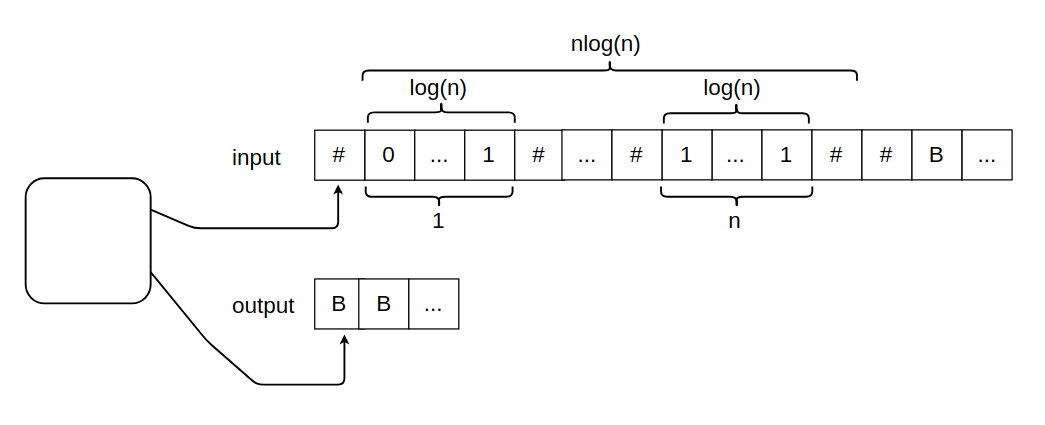
\includegraphics[width=\textwidth]{automa-permutazione}
\end{figure}

Assumiamo che la macchina abbia a disposizione due nastri, uno da cui legge e uno su cui scrive la permutazione; come sappiamo, questa assunzione non è vincolante, ma solo comoda per una descrizione ad alto livello. Assumiamo inoltre che i numeri siano memorizzati sul nastro come si vede in figura. Ogni numero occupa $log(n)$ celle in quanto codificato in binario, ed è separato dal successivo da un separatore $\#$. L'insieme è terminato da un doppio separatore $\#\#$.

\subparagraph{Fase di generazione}

La generazione \textit{non deterministica} della permutazione procede come segue:
\begin{enumerate}[label*=\arabic*.]
	\item se la testina del primo nastro si trova su un separatore (non di fine input) decide se copiare il numero che segue sul secondo nastro o meno:
	\begin{enumerate}[label*=\arabic*.]
		\item se decide di copiarlo:
		\begin{enumerate}[label*=\arabic*.]
			\item marca il primo separatore per ricordarsi che ha copiato il numero 
			\item avanza entrambe le testine scrivendo sul secondo nastro tutto ciò che legge sul primo
			\item quando incontra il separatore successivo, si ferma
		\end{enumerate}
		\item se decide di non copiarlo:
		\begin{enumerate}[label*=\arabic*.]
			\item avanza la testina sul primo nastro fino al separatore successivo, senza fare nulla
		\end{enumerate}
	\end{enumerate}
	\item se l'input è finito (doppio separatore), riporta la testina del primo nastro all'inizio
	\item torna al punto 1, ma se incontra un separatore marcato, avanza al separatore successivo senza toccare il secondo nastro
\end{enumerate}

Vediamo qual è la complessità di questa $NTM$. Assumendo che in ogni scansione decida di copiare almeno un numero (facilmente implementabile), questa effettua al massimo $n$ scansioni del nastro. Come evidenziato in figura, l'input è codificato su $nlog(n)$ celle, per cui ogni "copia" della macchina effettua $n^2 log(n)$ mosse nel generare una permutazione. La macchina quindi non deterministicamente le genera tutte in tempo polinomiale.

Sostituendo le codifiche di $\{1, ..., n\}$ con le codifiche di $\{ v_1, ..., v_n\}$ si ottiene un automa che calcola le permutazioni dei nodi necessarie per $T_{HP}$.

\subparagraph{Fase di verifica}

Le due verifiche possono essere effettuate in tempo polinomiale anche deterministicamente:
\begin{enumerate}[label*=\arabic*.]
	\item \begin{enumerate}[label*=\arabic*.]
		\item copia la codifica di $s$ sul secondo nastro
		\item porta la testina del primo nastro all'inizio di $v_1$, la testina del secondo nastro all'inizio di $s$
		\item avanza contemporaneamente le due testine, verificando l'uguaglianza cella per cella
		\item ripeti per $t$ e $v_n$
	\end{enumerate}
	Complessità logaritmica in $n$, ovvero polinomiale.

	\item Assumendo che gli archi siano codificati sul nastro come una sequenza di coppie di vertici $(u, w)$, si procede così:
	\begin{enumerate}[label*=\arabic*.]
		\item ripeti per ogni $v_i, v_{i+1}$ nella permutazione:
		\begin{enumerate}[label*=\arabic*.]
			\item ripeti per ogni arco $(u, w) \in E$:
			\begin{enumerate}[label*=\arabic*.]
				\item copia la codifica di $(v_i, v_{i+1}) \in permutazione$ all'inizio del secondo nastro, come se fosse un arco
				\item porta la prima testina all'inizio della codifica di $(u, w)$
				\item porta la seconda testina all'inizio della codifica di $(v_1, v_2)$
				\item confronta cella per cella le codifiche di $(u, w)$ e $(v_i, v_{i+1})$ finché non arrivi alla fine della codifica
				\item riporta la testina sul secondo nastro all'inizio del nastro
			\end{enumerate}
		\end{enumerate}
	\end{enumerate}
	Al più gli archi possono essere $n^2$, perciò la porzione da scandire è lunga $n^2 log n$. Si effettuano $n$ scansioni, per cui la complessità è $n \cdot n^2log(n) = n^3 log(n)$, ovvero polinomiale.
\end{enumerate}
Notiamo quindi che l'unica \textit{fase non deterministica} è la \textit{fase di generazione}, mentre la \textit{fase di verifica} può essere effettuata deterministicamente in tempo polinomiale.

\subsubsection{Problema del Clique}
Dato un grafo qualsiasi $G$, un $k$-clique è un sottoinsieme $C$ dei suoi vertici tale che ogni vertice è connesso con ogni altro
\[
	v_i, v_j \in C \implies \{v_i, v_j\} \in E
\]
Il problema del Clique consiste, dato un grafo, nel trovare il clique di cardinalità massima. Esso non è dunque un problema di \textit{decisione}, bensì un problema di \textit{ottimizzazione}. Consideriamo tuttavia il problema di decisione associato, parametrizzando per la cardinalità $k$ del clique cercato:

\[
	CLIQUE(k) = \{ <G, k> \ | \ G \text{ è un grafo con un } k\text{-clique} \}
\]
Il problema di ottimizzazione può quindi essere risolto sfruttando il problema di decisione, nel seguente modo:
\IncMargin{1em}
\begin{algorithm}
\SetKwInOut{Input}{input}\SetKwInOut{Output}{output}

\Input{Un grafo $G$}
\Output{La cardinalità della clique di cardinalità massima}
\BlankLine
\For{i = n $\to$ 1}{
	\If{$<G, i> \in CLIQUE(k)$}{
		\Return i\;
	}
}
\end{algorithm}\DecMargin{1em}

\newpage

Come prima, esibiamo una $NTM$ che decide $CLIQUE(k)$ in tempo \\
polinomiale:
\\

$T_{C}$
\begin{description}
	\item \textit{input}: $<G, k>$
	\item \textit{output}: SÌ se $<G, k> \in CLIQUE(k)$, NO altrimenti
	\item \textit{descrizione}:
	\begin{enumerate}[label*=\arabic*.]
		\item genera non deterministicamente un sottoinsieme $S$ \textit{qualunque} dei nodi di $G$

		\item verifica che $S$ sia un $k$-clique, ovvero:
		\begin{enumerate}[label*=\arabic*.]
			\item $|S| = k$
			\item $u, v \in S \implies \{u, v\} \in E$
		\end{enumerate}
	\end{enumerate}
\end{description}

\paragraph{Complessità}

Un automa che genera sottoinsiemi è molto simile a quello che genera permutazioni, descritto precedentemente: l'automa per ogni nodo sul primo nastro decide non deterministicamente se copiarlo o meno sul secondo nastro, in un'unica scansione. Così una "copia" dell'automa, andando con la testina su $v_1$, deciderà di copiarlo, decidendo invece di non copiare nessun altro nodo; un'altra invece deciderà di copiare ogni nodo, e così via.
\\

Ogni copia della macchina effettua un'unica scansione del nastro, che per quanto detto prima richiede $nlog(n)$ mosse. Ne consegue che anche in questo la complessità della \textit{fase non deterministica} è polinomiale. La \textit{fase di verifica}, similmente al problema del cammino hamiltoniano, può essere eseguita \textit{deterministicamente} in tempo polinomiale. 

\subsection{Verificatore polinomiale}

Nei due esempi precedenti si è visto come la \textit{fase di verifica} potesse essere eseguita \textit{deterministicamente} e in tempo \textit{polinomiale}. È quindi lecito chiedersi se questa sia una proprietà comune a tutti i problemi $NP$. Questo permetterebbe una definizione dei problemi $NP$ che ignora completamente il concetto del non determinismo. 

Introduciamo formalmente il concetto di \textit{verificatore}:
\begin{gather*}
	V \in TM \ verifica \ A \text{ se} \\
	A = \{ w \ | \ (w, c) \in L(V) \text{ per un qualche } certificato \ c \}
\end{gather*}
L'aggiunta di \textit{polinomiale} significa che il verificatore opera in una serie polinomiale di passi, cioè $t_V(n) = O(n^k)$.\\
Un \textit{certificato} è una possibile soluzione di una istanza di un problema, un concetto meglio comprensibile tramite un esempio. 
\\
Forniamo a tale scopo un verificatore per il problema di decisione $CLIQUE(k)$.
\\

$V_{CLIQUE}$:
\begin{description}
	\item \textit{input}: $(<G, k>, c)$
	\item \textit{output}: SÌ se $c$ è un $k$-clique di $G$, NO altrimenti
	\item \textit{descrizione}: semplicemente effettua la verifica esposta in precedenza
\end{description}

Come si vede, è più comodo esibire un verificatore rispetto ad esibire una $NTM$ che decide un problema. Vediamo un altro esempio.

\subsubsection{Problema dei numeri composti}
Istanze sì del problema sono tutti quei numeri \textit{composti}, ovvero non primi, per cui si riesce a trovare un naturale diverso da $1$ e da sè stesso che lo divide.
\[
	COMPOSITES = \{ p \ | \ p \in \mathbb{N} \text{ e } \exists \ q, r \in \mathbb{N} \text{ con } p = q \cdot r \text{ con } q \neq 1, q \neq n\}
\]

Esibiamo sia un $T_{COMP} \in NTM$ che lo decide, sia un verificatore $V_{COMP}$ che lo verifica.
\begin{itemize}
	\item $T_{COMP}$
	\begin{description}
		\item \textit{input}: $p \in \mathbb{N}$
		\item \textit{output}: SÌ se $p$ è composto, NO altrimenti
		\item \textit{descrizione}:
		\begin{enumerate}
			\item genera non deterministicamente tutti i naturali $q$ con $1 < q < p$

			\item verifica se $p \ mod \ q \equiv 0$
		\end{enumerate}
	\end{description}

	\item $V_{COMP}$
	\begin{description}
		\item \textit{input}: $(p, c)$ con $p, c \in \mathbb{N} $
		\item \textit{output}: SÌ se $c$ divide $p$, NO altrimenti
		\item \textit{descrizione}:
		\begin{enumerate}
			\item verifica se $c \neq 1$ e se $c < p$
			\item verifica se $p \ mod \ c \equiv 0$
		\end{enumerate}
		
	\end{description}
\end{itemize}
Anche questo problema sta in $NP$, e anche in questo caso siamo riusciti ad esibire un verificatore polinomiale. Come accennato precedentemente, questa è effettivamente una proprietà comune a tutti i problemi in $NP$.

\subsection{Dimostrazione NP = VP}

Definiamo $VP = \{ L \ | \ \exists \text{ verificatore polinomiale } V \text{ che verifica } L \}$. La dimostrazione, come di consueto, procede per \textit{doppia inclusione}.


\paragraph{NP $\subseteq$ VP}

Vogliamo mostrare che $L \in NP \implies \exists V \in VP \text{ che lo verifica}$.
\\
\\
Se $L \in NP$ allora per definizione $\exists T \in NTM$ con $t_T(n) = O(n^k)$, per qualche $k$, tale che $L(T) = L$. Costruiamo un verificatore per $L$.

Supponiamo che l'albero di computazione di $T$ abbia massimo grado di non determinismo uguale a 2. Inoltre, come visto in precedenza, esso sarà alto $t_T(n)$.
Costruiamo allora un certificato $c \in \{ 0, 1 \}^{\star}$, con $|c| = t_T(n)$. Un certificato del genere è in grado di identificare univocamente ogni cammino radice foglia, ovvero un percorso di computazione. Il verificatore $V_L$ è allora così composto:
\begin{description}
	\item \textit{input}: $<w, c>$
	\item \textit{descrizione}:
	\begin{enumerate}
		\item esegui $T$ su $x$ seguendo il percorso di computazione identificato da $c$
		\item se $T$ accetta, allora accetta
		\item se $T$ rifiuta, allora rifiuta
	\end{enumerate}
\end{description}

La costruzione del verificatore è corretta perché possiamo esprimere $L(T)$ secondo la definizione di verificatore:
\[
	L(T) = \{w \ |\ <w, c > \in L(V_L) \text{ per qualche certificato } c \}
\]
Infatti per ogni parola $w$ accettata da $T$ esiste almeno un cammino di accettazione per $w$, dunque per costruzione esiste un
certificato $c$ per cui $V_L$ accetta. 
\\
Se invece $w$ è rifiutata da $T$, allora nessun cammino è di accettazione, quindi nessun certificato identifica un cammino di accettazione, quindi $V_L$ rifiuta $<w, c>$ per qualsiasi certificato $c$.
\\
Inoltre la complessità è polinomiale perché la sequenza $c$ è di lunghezza polinomiale, e quindi anche il numero di passi di $T$ che $V_L$ simula è polinomiale.

\paragraph{VP $\subseteq$ NP} 

Vogliamo mostrare che $L \in VP \implies \exists T \in NP \text{ che lo decide}$.
\\
\\
Se $L \in VP$ allora per definizione $\exists V$ tale che $ L = \{ w \ | \ <w, c> \in L(V)\}$ con $t_V(n) = O(n^k)$. Costruiamo una $T_L \in NTM$ che decide $L$.

\newpage

$T_L$
\begin{description}
	\item \textit{input}: $w$ 
	\item \textit{output}: SÌ se $x \in L$, NO altrimenti
	\item \textit{descrizione}:
	\begin{enumerate}[label*=\arabic*.]
		\item genera non deterministicamente tutti i certificati $c$ con $|c| \leq t_V(n)$

		\item esegui il verificatore su $<x, c>$
		\begin{enumerate}[label*=\arabic*.]
			\item se $V$ accetta, allora accetta
			\item se $V$ rifiuta, allora rifiuta
		\end{enumerate}
	\end{enumerate}
\end{description}

La costruzione è corretta in quanto se $w \in L$ allora esiste almeno un certificato $c$ per cui $V$ accetta $<w, c>$. Poiché $T_L$ genera non deterministicamente \textit{tutti} i certificati, necessariamente genera anche $c$, e un suo cammino di computazione esegue $V$ su $<w, c>$, il quale per quanto detto prima accetta, e quindi esiste un cammino di accettazione di $T_L$ per $w$.
\\
Se invece $w \notin L$ allora non esiste un certificato $c$ per cui $V$ accetta $<w, c>$. Quindi per \textit{nessun} certificato generato da $T_L$ si avrà l'accettazione di $V$ su $<w, c>$. Ne segue che non esiste un cammino di accettazione di $T_L$ per $w$, ovvero $T_L$ rifiuta $w$.
